%--------------------------------------------------------------------------------------------------
% 
\chapter{Heterogeneous Streaming Sources Data Fusion for Machine Learning}
\label{ch:data-fusion}
%--------------------------------------------------------------------------------------------------

%================================================
% OVERVIEW
%================================================

%\section{Overview}
%\section{Architecture}
%\section{Implementation in a Cloud}
%\section{Implementation on an Edge System}

Vmes je treba dat kak Chapter, v katerem ima vsak svoj nek manjši uvod. 
Potem naslov članka in kje je bil objavljen. 

This section presenta a paper TITLE, avtorji. The paper was first published by. The final manuscript was published in ... 

Čisto kratek uvod preden pride članek. Povezava med naslovom članka in naslovom poglavja.


Najboljše vprašati na MPŠ!
Vse reference iz člankov na koncu doktorata.
Index of figures.

\begin{list}{}
{\leftmargin=2.5em \itemindent=-2.5em}
    \item K. Kenda, B. Kažič, E. Novak, and D. Mladenić, “Streaming data fusion for the internetof things,” \textit{Sensors}, vol. 19, no. 8, p. 1955, 2019.
\end{list}

\begin{quote}
    \textit{Klemen Kenda is the main author of the paper. He contributed to conceptualization, methodology, software development, validation, formal analysis, data curation, writing, visualization, project administration and funding acquisition.}
\end{quote}

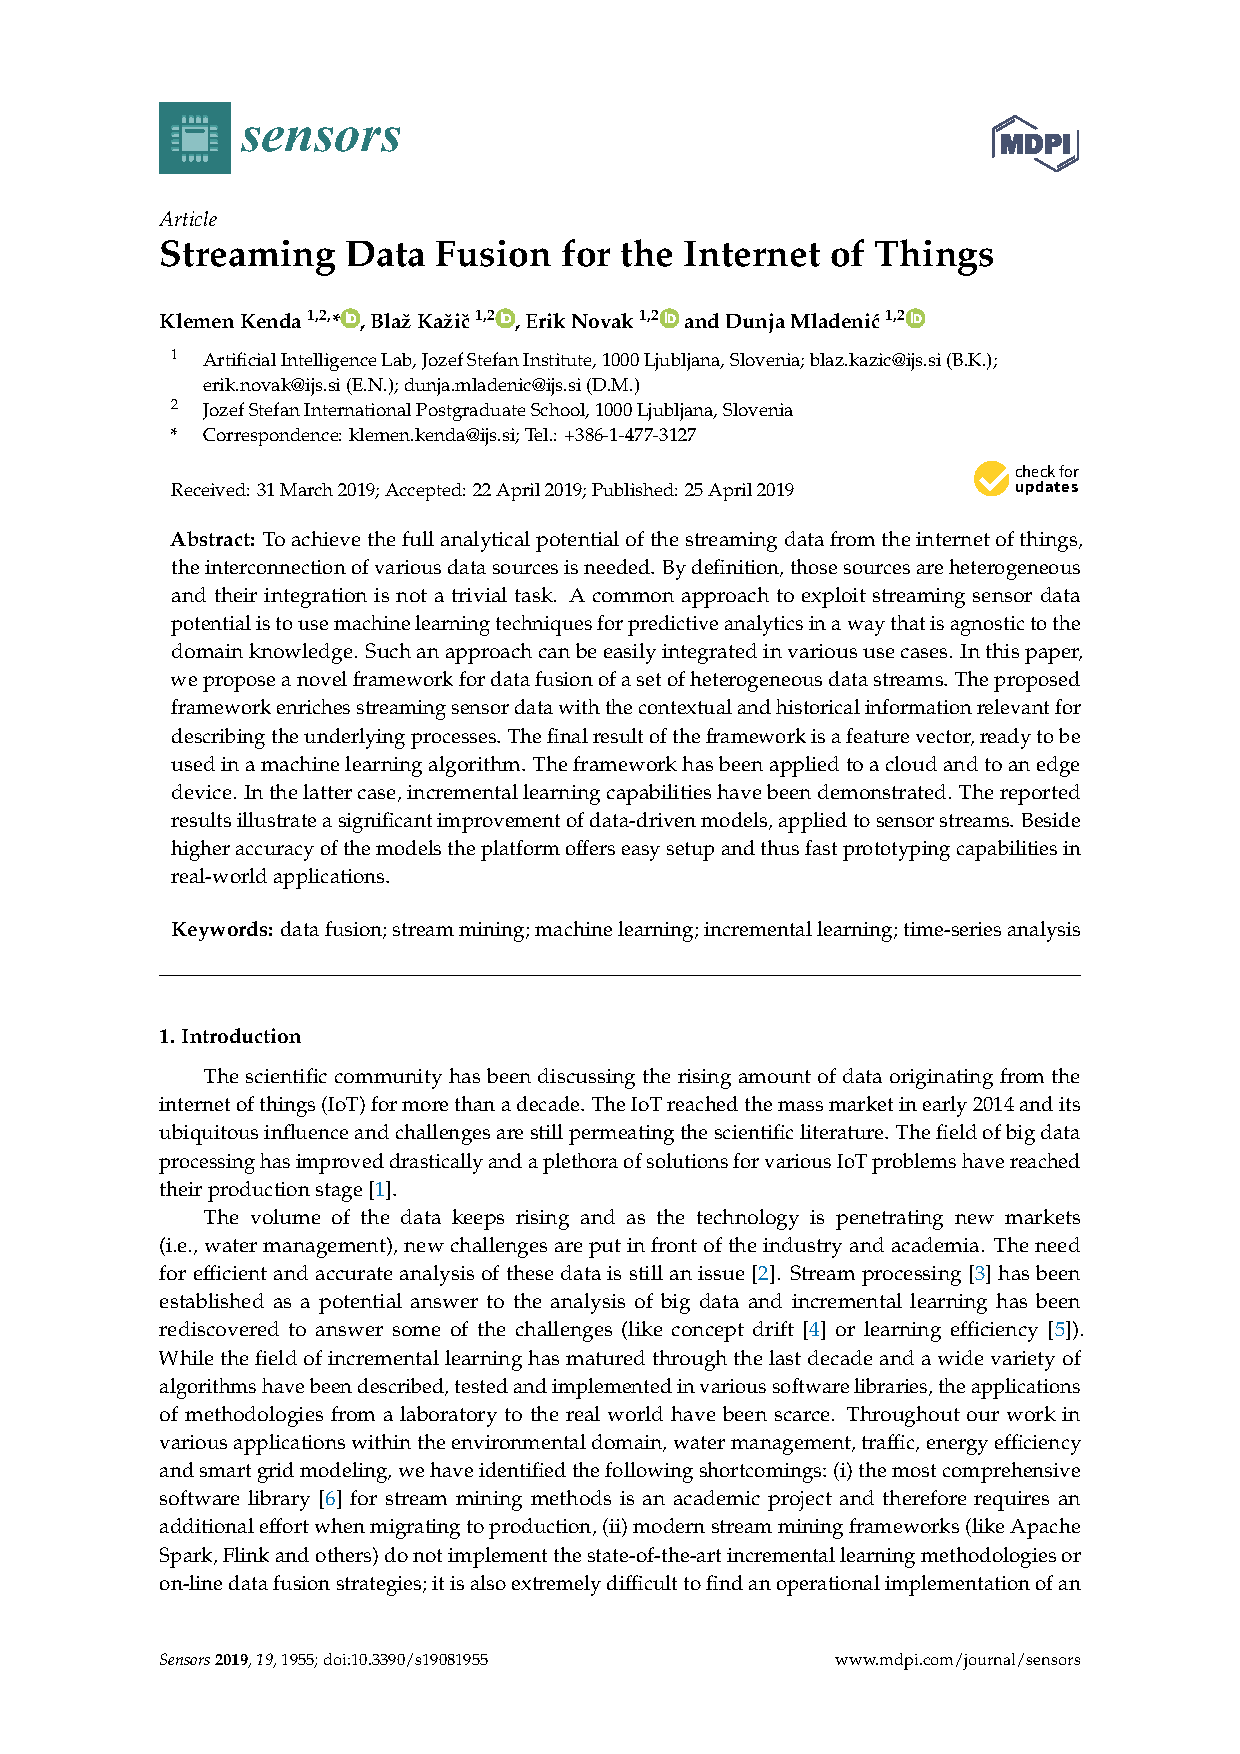
\includepdf[pages=-]{papers/streaming_data_fusion_for_iot.pdf}